\documentclass[12pt]{article}
\usepackage{amsmath}
\usepackage{amssymb}
\usepackage{geometry}
\usepackage{graphicx}
\usepackage{cite}
\usepackage{url}

\bibliographystyle{ieeetran}

%opening
\title{Expose on the SIAM Article 
	Improved prediction of antibiotic resistance: learning from the data}
\author{Darja Strahlberg}

\begin{document}

\maketitle

\section{Introduction}
\subsection{Motivation}
Antibiotic Resistance is a rising problem in the modern world. Bacterial infections, for example like pneumonia, meningitis,  are commonly treated through antibiotic therapy applied to individuals. Knowing the frequency of the spread may help to creat a reaction scheme. The antimicrobial-drug resistance has many concerns like its economic impact on physicians, patients, health-care administrators, pharmaceutical producers, and the public.~\cite{JohnE.McGowan.2001}
Machine Laerning models and Big Data offer new approach on the prediction of the antibiotic resistance. Machine Learning methods can be integrated into the solving high dimensional models, where standard mathematics cannot help. 

The classical SIR Model (math) has a disadvantage, that it does not consider randomness in the prediction, so making the model less robust. AR (Autoregressive) models use history data to make a future predictions. It usually requires very little data, so it is very useful in the epidemiological models.

The current research, using the ML methods, is concentrated on the on Antimicrobial resistance gene detection. So it is the resistome prediction. We are asking a question is it possible to predict the spread pattern of the antibiotic resistance? Is it important?

The central hypothesis states, that machine learning method will provide more accurate prediction of the spread of antibiotic resistance. It has a randomness factor (although we do not know how the machine learning), additionally, we can use additional data, like the amount of sick people, time of spread of the resistance, the amount of consumed antibiotics?

There are different ways to investigate the development of the antibiotics resistance. For example, withing the patient, a hospital or a community. We have a goal to look at the spread of the resistance in the community globally.~\cite{Austin.} The current research, using the ML methods, is concentrated on the on Antimicrobial resistance gene detection. So it is the resistome prediction. We are asking a question is it possible to predict the spread pattern of the antibiotic resistance? Is it important?

\begin{figure}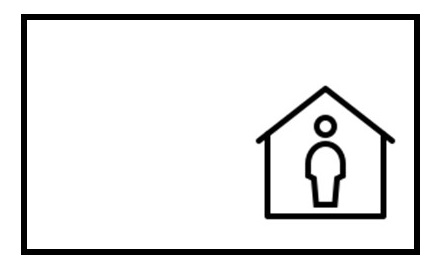
\includegraphics[width=\textwidth]{Images/distribution.jpg}\caption{Different levels to predict the spread of antibiotic resistance: withing a patient, a hospital or a community.}
	\end{figure}


\subsection{Historical Overview}
There was observed a shift in the developed world, that the mortality from infectious diseases had been replaced by mortality from chronic illnesses such as heart disease, cancer and stroke. It lead to the fact that pharmaceutical companies stopped spending resources on the development of the new antibiotics, but instead on the medicine to cure other diseases. By the end of the twentieth century, in most of the developed world, mortality from infectious diseases had been replaced by mortality from chronic illnesses such as heart disease, cancer and stroke~\cite{Dasbas.2016}
Table?
It is importnat to show the statistics on death rate from infectious deseases in Germany and the EU

\subsection{Goal}

We can try to answer the question how the frequency of resistance changes over time. We want to provide a scenario analysis. 

The big data analysis can help answering following questions: surveillance, hypothesis-generating research, and causal inference.~\cite{Mooney.2018}

Antibiotic consumption has a direct influence on the frequency of resistance in communities. It is seen as difficult due to the lack of the recorded data. So the machine learning approach can give a new life to the prediction of the antibiotic resistance.~\cite{Austin.}
The temporal nature of epidemiology data and the need for real-time prediction by the system makes the problem residing in the category of time-series forecasting or prediction.~\cite{Cho.03.06.2014b} There is also an issue with the time delay in the epidemiological data. So the good prediction can make a difference~\cite{Harvard.}

Additionally it is important to include the number of sick people of the disease. Pay attention to the correlation.
Antibiotic consumption has a direct influence on the frequency of resistance in communities. It is seen as difficult due to the lack of the recorded data. So the machine learning approch can give a new life to the prediction of the antibiotic resistance.~\cite{Austin.}
The idea is to include additional data to broader analysis of bacterial fitness, infection dynamics, horizontal gene transfer and other factors.~\cite[S.~689]{Sommer.2017b}
Big Data should satisfy three characteristics: high volume and high variety data, high velocity feedback mechanisms.~\cite{Mooney.2015}

- factors that influence the evolution of antibiotic resistance and discuss these factors in the context of early drug discovery - paths for a resistance to be developed: vertical evolution, horizontal evolution.
\textbf{Acinetobacter baumannii, }carbapenem-resistant
\textbf{Pseudomonas aeruginosa, }carbapenem-resistant \textbf{Enterobacteriaceae*, }carbapenem-resistant, 3rd generation cephalosporin-resistant~\cite{Tacconelli.}

\section{Results and Discussion}
\subsection{Biological Overview: two ways of the spread}
he traditional desease reporting istaking several steps. Public informs their Healthcare workers, they inform Laboratories, they Minister of Health and the World bodies, like WHO.~\cite{Harvard.}
Resistance genes produce enzymes that either modify or eliminate an antibiotic. Resistance genes can be spread by vertical transmission from parent to offspring or by horizontal transfer between different strains and species of bacteria. Sensitive microbes become resistant to antibiotics either through the acquisition of plasmidborne resistance genes or through mutations that either upregulate the expression of a resistance gene or alter the binding or substrate specificity of an enzyme encoded by a resistance gene.~\cite[S.~1237]{Barlow.2003}

\begin{figure}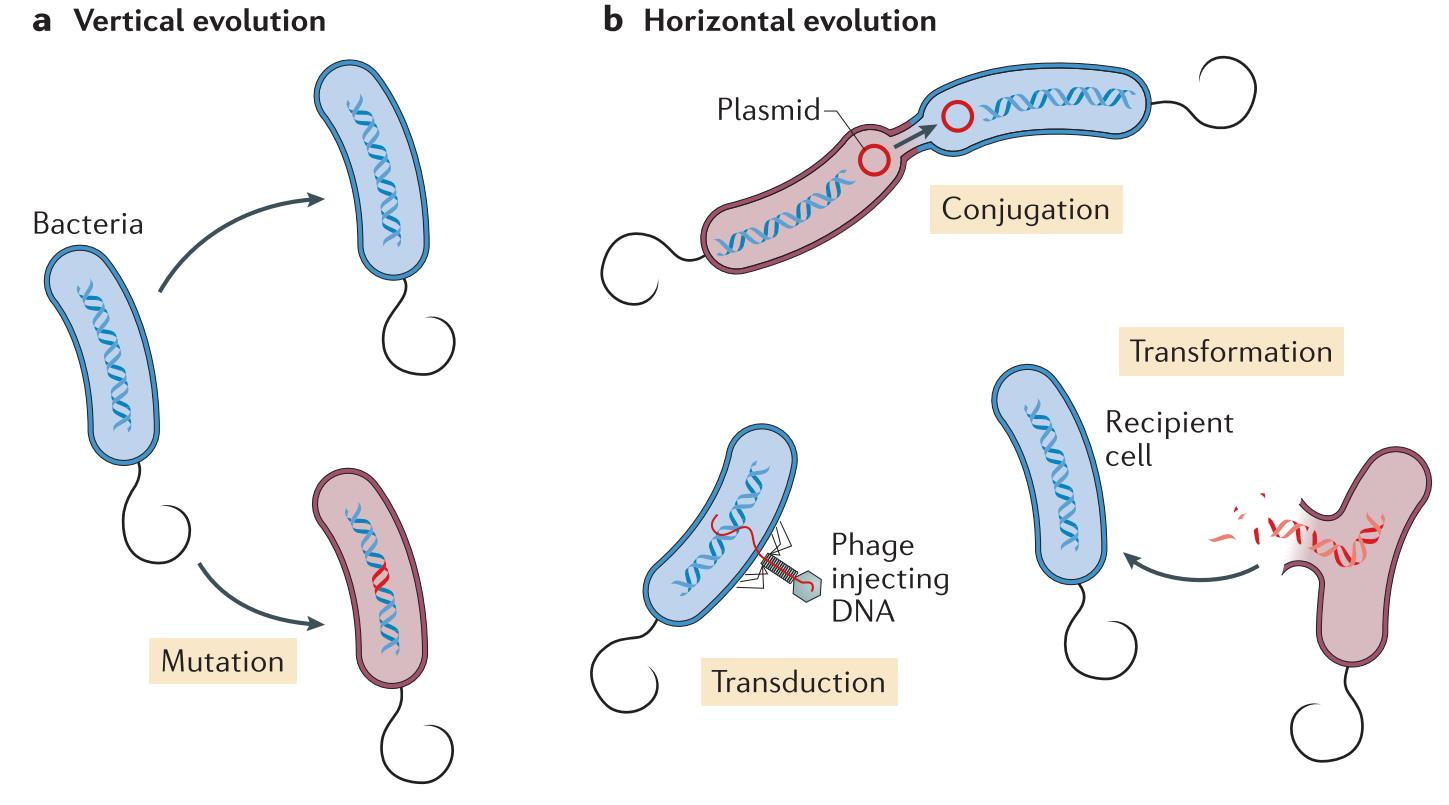
\includegraphics[width=\textwidth]{Images/f65b4498-79f9-47f3-badf-19f7b1ec7312.jpg}\caption{Evolution of resistance. Sommer, Munck et al. 2017 - Prediction of antibiotic resistance.jpg}
	~\cite[S.~690]{Sommer.2017b}\end{figure}

\subsection{Math Method of Linear Regression}
Autoregressive (AR) models have been most popular for time series forecasting [6, 8]. The basic idea is to model the future state as a linear combination of past data points.~\cite{Cho.03.06.2014b}
While being intuitive and popular, such models have limited prediction power due to the rather narrow function space, lack ofthe ability to model individuallevel information, and do not embrace new developments in recent machine learning and data mining technologies.~\cite{Cho.03.06.2014b}
\subsection{ML Method}
Machine learning is an umbrella term for techniques that fit models algorithmically by adapting to patterns in data~\cite{Mooney.2018}
We adopt Recurrent Neural Networks (RNNs) to capture the long-term correlation in the data and Convolutional Neural Networks (CNNs) to fuse information from data of different sources. A residual structure is also applied to prevent overfitting issues in the training process.~\cite{Cho.03.06.2014b}
We employ an recurrent neural network (RNN) module to capture the temporal dependencies in the data. Specifically, we utilize an Gated Recurrent Unit (GRU) [2] in our framework. The input data are passed through a gate, which is then used to compute the new state in the memory cell ofGRU given the old value.~\cite{Cho.03.06.2014b}
a CNN for capturing correlation between signals, a RNN for linking up the dependencies in the temporal dimension and the residual links for fast training and overfitting prevention. We carefully restrain the parameter space, making the total model have a similar size as AR.~\cite{Cho.03.06.2014b}
We have measured the amount of people with the antibiotic resistance?

\section{Conclusion}
Hopefully, we have proved the hypothesis that Machine Learning approach gives a better prediction, and that more data contribute to it. 
Why does it make a difference?

\bibliography{References}



\end{document}